\chapter{Basic Theory}

\setcounter{section}{1}
\setcounter{subsection}{0}
\subsection{}\label{part1-sec1.1} \pageoriginale

We shall develop in this course Nevanlinna's theory of meromorphic
functions. This theory has proved a tool of unparallelled precision
for the study of the roots of equations $f(z)=a$, $f^{(1)}(z)=b$,
etc.\@ whether single or multiple and their relative frequency. Basic
to this study is the Nevanlinna Characteristic $T(r)$ which is an
indication of the growth of the function $f(z)$. We shall see in
Theorem \ref{thm2} that for every a $T(r)$ is, apart from a bounded
term, the sum of two components $m(r,a)+N(r,a)$ of which the second
measures the number of roots of the equation $f(z)=a$ in $|z|<r$ and
the first the average closeness of $f(z)$ to a on $|z|=r$. The second
fundamental theorem shows that in general the second term dominates
and many applications giving well beyond Picard's theorem result.

\subsection{The Poisson-Jensen Formula}

We shall start with Poisson-Jensen formula which plays a fundamental
role in our study.

\begin{thm}\label{thm1}
If $f(z)$ is meromorphic in $|z|\leq R$ and has there zeros $a_{p}$
and poles $b_{\nu}$ and if $\zeta=re^{i}$, $f(\zeta)\neq 0$, then for
$0\leq r\leq R$ we have
\begin{align*}
\log f(re^{i\theta}) &=
\frac{1}{2\pi}\int\limits^{2\pi}_{0}
\frac{\log|(Re^{i\phi})|(R^{2}-r^{2})dr}{R^{2}-2Rr\cos \,(\phi-\theta) +
  r^{2}} + \sum_{\mu}\log\left|
\frac{R(\zeta-a_{\mu})}{R^{2}-\ob{a}_{\mu}\zeta}\right|\\ 
& \quad - \sum_{\nu}\log\left |
\frac{R(\zeta-b_{\nu})}{R^{2}-\ob{b}_{\nu}\zeta}
\right|\tag{1.1}\label{part-eq1.1} 
\end{align*}
\end{thm}

\begin{proof}
Let\pageoriginale $f(z)\neq 0$, in $|z|\leq 1$. Then, since we can
define an analytic branch of $\log f(z)$ in $|z|\leq 1$, we have by
the residue theorem
$$
\frac{1}{2\pi i}\int\limits_{|z|=1}\log f(z)\frac{dz}{z}=\log f(0) 
$$
By change of variable,
$$
\frac{1}{2\pi}\int\limits^{2\pi}_{0}\log f(e^{i\phi})d\phi=\log f(0) 
$$ 
and now taking real part on both sides
$$
\frac{1}{2\pi}\int\limits^{2\pi}_{0}\log |f(e^{i\phi})|d\phi=\log|f(0)| 
$$
For any $\zeta$ with $|\zeta|<1$, we effect the conformal
transformation $w=\dfrac{z-\zeta}{1-\ob{\zeta}z}$ for the integral
$\int\limits_{|z|=1}\log f(z)\dfrac{dz}{z}$. This in turn becomes,
$$
\frac{1}{2\pi i}\int\limits_{|w|=1}\log \varphi(w)\dfrac{dw}{w}=\log
f(\zeta)\text{ \ where \ } \varphi(w)=f\{z(w)\}
$$
so that $\varphi(0)=f(\zeta)$. Substituting in the integral
$z=e^{i\phi}$ and taking real part we get,
$$ 
\frac{1}{2\pi}\int\limits^{2\pi}_{0}\frac{\log|f(e^{i\phi})|}{1-2r\cos
  (\phi-\theta)+r^{2}}(1-r^{2})\,d\phi=\log|f(\zeta)|,\zeta=re^{i\theta} 
$$
\end{proof}

Now for the function $f(z)$ with poles $b_{\nu}$ and zeros $a_{\mu}$
none of them being on $|z|=1$, let us define
$$
\psi(z)=f(z)\frac{\pi\dfrac{(z-b_{\nu})}{(1-\ob{b}_{\nu}z)}}{\pi\dfrac{(z-a_{\mu})}{(1-\ob{a}_{\mu}z)}}
$$
On\pageoriginale $|z|=1$, $|\psi(z)|=|f(z)|$ and the function has no
zeros or poles in $|z|\leq 1$. By the above result,
\begin{gather*}
\frac{1}{2\pi}\int\limits^{2\pi}_{0}\log|\psi(e^{i\theta})|\frac{(1-r^{2})}{1-2r\cos(\phi-\theta)+r^{2}}d\phi=\log|\psi(\zeta)|\\
\zeta=re^{i\theta},r<1
\end{gather*}
Substitution for $\psi$ gives the theorem for $R=1$. In the case when
there are poles and zeros on the circumference of the unit circle we
proceed as follows. We have only to show that if $f(z)$ has no zeros
or poles in $|z|<1$, but has poles and zeros on $|z|=1$, then
$$
\frac{1}{2\pi i}\int\limits_{|z|=1}\log f(z)\frac{dz}{z}=\log f(0)
$$
For if $f(z)$ has zeros and poles in $|z|<1$ we can consider
$\psi(z)$, in place of $f(z)$. Further we can assume that there is
only one zero (the case of pole being treated in the same manner) on
$|z|=1$. For the case when $f(z)$ has a finite number (it can have at
most only a finite number) of zeros (poles) can be treated similarly.

Let therefore $z=a$, $|a|=1$ be a zero of $f(z)$ on $|z|=1$. Let $P$
be the point $z=a$ and consider a circle of radius $\rho<1$ about $P$,
$\rho$ being small. Consider the contour $SQR$ (fig.)
Inside it $f(z)$ has no zeros or poles. Hence by the residue theorem,
$\int\limits \log f(z)\, dz=\log f(0)$. Thus it is enough to prove that
$\int\limits_{QR}\log f(z)\,dz$ tends to zero as $\rho$ tends to zero.
\begin{figure}[H]
\centering
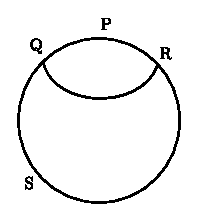
\includegraphics{hayman_fig1.eps}
\end{figure}

Let $z=a$ be zero of order $k$. Then $f(z)=(z-a)^{k}\lambda(z)$,
$\lambda(a)\neq 0$, in a certain neighbourhood of $a$; and
we\pageoriginale can assume the choice of $\rho$ such that this
expansion is valid within and on the circle of radius $\rho$ about
$P$.
$$
\int\limits_{QR}\log f(z)\dfrac{dz}{z}=k\int\limits_{QR}\log(z-a)\frac{dz}{z}+\int\limits
\log \lambda(z)\frac{dz}{z}
$$
Since $\lambda(z)$ remains bounded the second integral tends to
zero. So we have only to prove that $\int\limits_{QR}\log(z-a)\dfrac{dz}{z}$
tends to zero as $\rho\to 0$, Now,
\begin{align*}
\left| \int\limits_{QR}\log (z-a)\frac{dz}{z}\right| & \leq \max
\left\{\left|\dfrac{\log |(z-a)|}{|z|}\right|\right\}\\
\pi\rho & \leq [\log
  (1/\rho)+0(1)]\pi \rho\to 0 \text{ \ if \ } \rho\leq \frac{1}{2}
\end{align*}
This proves the result, in the case when the function $f(z)$ has zeros
or poles on the unit circle. In case $R\neq 1$, we consider the
function $f(Rz)$ instead of $f(z)$ and arrive at the result. Hence the
theorem is proved completely.

\begin{coro*}
In the special case when $\zeta=0$ we get the Jensen's formula
\begin{equation*}
\log
|f(0)|=\frac{1}{2\pi}\int\limits^{2\pi}_{0}\log|f(Re^{i\phi})|d\phi+\sum_{\mu}\log\left|\frac{a_{\mu}}{R}\right|-\sum_{\nu}\log\left|\frac{b_{\nu}}{R}\right|\tag{1.2}\label{part1-eq1.2} 
\end{equation*}
the summation ranging over poles and zeros of $f(z)$ in $|z|\leq
R$. The above formula does not hold if zero is a pole or a zero of
$f(z)$. If $f(0)=0$ or $\infty$ and $f(z)$ is not identically constant
then $f(z)=C_{\lambda}z^{\lambda}+\cdots+\cdots$. Consider
$f(z)/z^{\curlyvee}$. This has neither zero nor pole at zero. Hence we
get,
\begin{align*}
\log |C_{\lambda}| &=
\frac{1}{2\pi}\int\limits^{2\pi}_{0} \log\left|
\frac{f(Re^{i\phi})}{R^{\lambda}}\right|d\phi+\sum 
\log \frac{|a_{\mu}|}{R}-\sum\log \frac{|b_{\nu}|}{R}\\
&=\frac{1}{2\pi}\int\limits^{2\pi}_{0}\log|f(Re^{i\phi})|
d\phi+\sum\log\frac{|a_{\mu}|}{R}-\sum 
\log \frac{|b_{\nu}|}{R}-\lambda\log R
\end{align*}
where\pageoriginale sums are taken over zeros and poles of $f(z)$ in
$0\leq |z|\leq R$.
\end{coro*}

\subsection{The Characteristic Function}\label{part1-sec1.3}

Set for $x$, real and positive,
\begin{align*}
\log^{+}x &= \log x\text{ \ if \ } x>1,\\
\log^{+}x &= 0\qquad\text{if \ } x \leq 1,
\end{align*}
Then clearly $\log x=\log^{+}x-\log^{+}(1/x)$. So
$$
\int\limits^{2\pi}_{0}\log|f(Re^{i\phi})|d\phi=\int\limits^{2\pi}_{0}\log^{+}|f(Re^{i\phi})|d\phi-\int\limits^{2\pi}_{0}\log^{+}\frac{1}{|f(Re^{i\phi})|}d\phi
$$
We note that the first term represents the contribution when $f$ is
large and the second term when $f$ is small.

Let $0<r_{1}\leq r_{2}\leq \ldots\leq r_{n}\leq R$ be the moduli of
the poles in the order of increasing magnitude. Let $n(r)$ denote the
number of poles in $|z|<r$ of $f(z)$. Then the Riemann-Stieljes'
integral,
$$
\int\limits^{R}_{0}\log \frac{R}{t}dn(t)=\sum_{\nu}\log\frac{1}{|b_{\nu}|}
$$
given on integrating by parts,
$$
\left. n(t)\log
\frac{R}{t}\right]^{R}_{0}+\int\limits^{R}_{0}n(t)\frac{dt}{t}=\sum_{\nu}\log(R/|b_{\nu}|) 
$$
The first term is zero, in consequence of the fact $n(t)=0$, near
zero.

We write $n(r,f)$ for the number of poles of $f(z)$ in $|z|\leq r$, so
that $n(r,1/f)$ is equal to the number of zeros of $f(z)$ in $|z|\leq
r$. We define $N(r,f)$ to be
\begin{equation*}
\int\limits^{r}_{0}n(t,f)\frac{dt}{t}\tag{3}\label{part1-eq3}
\end{equation*}
If\pageoriginale $f(0)=\infty$ we define
$N(r,f)=\int\limits^{r}_{0}[n(t,f)-n(0,f)]\dfrac{dt}{t}+n(0,f)\log r$. Then
the formula \eqref{part1-eq1.2} becomes, for $f(0)\neq 0$, $\infty$
\begin{gather*}
\log
|f(0)|=\frac{1}{2\pi}\int\limits^{2\pi}_{0}\log^{+}|f(re^{i\theta})|d\theta-\frac{1}{2\pi}\int\limits^{2\pi}_{0}\log^{+}\frac{1}{|f(re^{i\theta})|}d\theta+N(r.f)\\
-N(r,1/f).
\end{gather*}
We define,
\begin{equation*}
T(r,f)=N(r,f)+m(r,f)\tag{1.4}\label{part1-eq1.4}
\end{equation*}
where,
\begin{equation*}
m(r,f)=\frac{1}{2\pi}\int\limits^{2\pi}_{0}
\log^{+}|f(re^{i\theta})|d\theta\tag{1.5}\label{part1-eq1.5} 
\end{equation*}
Again \eqref{part1-eq1.2} takes the form, for $f(0)\neq 0$, $\infty$
\begin{equation*}
T(r,f)=T(r,1/f)+\log |f(0)|\tag{$1.2'$}\label{part1-eq1.2'}
\end{equation*}

If $f(z)\sim C_{\lambda}Z^{\lambda}$ near $z=0$, where $\lambda\neq
0$, then we obtain\break $T(r,f)=T(r,1/f)+\log|C_{\lambda}|$. In future such
modifications will be taken for granted.

The function $T(r,f)$ is called the {\em Characteristic Function} of
$f(z)$.

This is the Nevanlinna characteristic function.

\begin{thm}\label{thm2}
First fundamental theorem.
\end{thm}

For any finite complex $a$,
\begin{align*}
T(r,f)&=T[r,1/(f-a)]+\log |f(0)-a|+\epsilon(a)\\
&\qquad\qquad\text{ \ where \ }|\epsilon(a)|\leq \log^{+}|a|+\log 2.
\end{align*}

\begin{proof}
We note that $\log^{+}|z_{1}+z_{2}|\leq
\log^{+}z_{1}|+\log^{+}|z_{2}|+\log 2$ 

\smallskip
and \quad
$\log^{+}|z_{1}-z_{2}|\geq \log^{+}|z_{1}|-\log^{+}|z_{2}|-\log
2$. Whence,\pageoriginale
$$
\log^{+}|f(z)-a|-\log^{+}|f(z)|\leq \log 2+\log^{+}|a|
$$
Integrating we get,
$$
-\log 2-\log^{+}|a|+m(r,f-a)\leq m(r,f)\leq \log
2+\log^{+}|a|+m(r,f-a)
$$
Since $f$ and $f-a$ have the same poles,
$$
N(r,f)=N(r,f-a).
$$
Therefore,
$$
T(r,f-a)-\log^{+}|a|-\log 2\leq T(r,f)\leq \log 2+\log^{+}|a|+T(r,f-a)
$$
That is, $|T(r,f)-T(r,f-a)|\leq \log 2+\log^{+}|a|$
$$
T(r,f)+T(r,f-a)+\epsilon(a), \text{ \ where \ } |\epsilon(a)|\leq \log
2+\log^{+}|a| 
$$
From \eqref{part1-eq1.2'} we have,
$$
T(r,f)=T\left(r,\frac{1}{f-a}\right)+\log|f(0)-a|+\epsilon(a)
$$
where $|\epsilon(a)|\leq \log 2+\log^{+}|a|$.
Hence the theorem is proved.
\end{proof}

If we write $m(r,a)$, $N(r,a)$ for $m\left(r,\dfrac{1}{f-a}\right)$,
$N\left(r,\dfrac{1}{f-a}\right)$, then $m(r,a)$ represents the average
degree of approximation of $f(z)$ to the value a on the circle $|z|=r$
and $N(r,a)$ the term involving the numbers of zeros of
$f(z)-a$. Their sum can be regarded as the total affinity of $f(z)$
for the value $a$ and we see than apart from a bounded term the total
affinity for every value of $a$. However, the relative size of the two
terms $m$, $N$ remains in doubt. We shall see in the second
fundamental theorem that in general it is $N(r,a)$ that is the larger
component. The value of $a$ for which this is not the case will be
called exceptional.

%%1.3.1
\subsubsection{Let us now consider some
  examples}\label{part1-subsubsec1.3.1}\pageoriginale 

\begin{enumerate}
\item Let $f(z)=P(z)/Q(z)$, $P(z)$ and $Q(z)$ being polynomials of
  degrees $m$ and $n$ respectively, and prime to each other, that is
  have no common roots.

Then for large $r$, $|f(z)|\sim Cr^{m-n}$.

So if $m$ is greater than $n$, $m(r,f)=(m-n)\log r+0(1)$ and since
\begin{gather*}
\log^{+}x=0, \text{ \ for \ } 0<x\leq 1, m(r,1/f)=0\\
 \text{ \ and \ }\qquad m(r,1/(f-a))=0.\tag{1.6}\label{part1-eq1.6} 
\end{gather*}
for large $r$ and fixed $a$. Since $f(z)=\infty$ has $n$ roots in the
open plane, $n(t,f)=n$, for $t>t_{0}$ and $N(r,f)=n\log r+0(1)$. Again
$T(r,f)=m(r,f)+N(r,f)$ which is equal to $m\log r+0(1)$ for $\ub{a}$
finite again by \eqref{part1-eq1.6} and theorem \ref{thm2},
$N(r,1/(f-a))=m\log r+0(1)$, $\ub{a}$ finite. Thus
$\left[N\left(r,\dfrac{1}{f-a}\right)/T(r,f)\right]\to 1$ as $r\to
\infty$. In this case $a=\infty$ is the only exceptional value.

Similar conclusions follow if $m$ is less than $n$ by taking $1/f$ in
place of $f$ in the above discussion. In this case $a=0=f(\infty)$ is
the only exceptional value.

If $m$ is equal to $n$, $f=c+0(z^{-\lambda})$ (say). Or writing,
$f-c\sim b(z^{-\lambda})$, we see that $m(r,1/(f-c))=\lambda \log
r+0(1)$
\begin{align*}
m(r,1/(f-a)) &= 0(1), \text{ \ when \ } a\neq c\\
m(r,f) &= 0(1), N(r,f)=n\log r+0(1)
\end{align*}
Thus $T(r,f)=n\log r+0(1)$ and, 
\begin{align*}
N(r,a) &= n\log r+0(1), a\neq c\\
N(r,c) &= (n-\lambda)\log r+0(1).
\end{align*}
Thus in any case 
\begin{align*}
T(r,f) &= (\Max. \;\; m,n) \log r+0(1)\\
\text{\iec \ } T(r,f) &\sim (\Max. \;\; m,n)\log r.
\end{align*}\pageoriginale
Thus in the case of a rational function there is always only one
exceptional value, viz., $f(\infty)$

\item Let $f(z)=e^{z}$. In this case the value of $m(r,f)$ is,
\begin{align*}
m(r,f) &= 1/2\pi\int\limits^{2\pi}_{0}\log^{+}e^{r\cos \theta}d\theta\\
&= 1/2\pi\int\limits^{\pi/2}_{-\pi/2}\cos\theta \ d\theta\\
&= r/\pi
\end{align*}
because $\cos\theta\leq 0$ in $\pi/2\leq \theta\leq \pi$, $-3\pi/2\leq
\theta\leq -\pi/2$ and so $\log^{+}e^{r\cos \theta}$ is equal to zero.
\end{enumerate}

Since $e^{z}$ has no poles, $N(r,f)=0$. Consequently $T(r,f)$ is equal
to $m(r,f)$ which in turn is equal to $r/\pi$.

We employ the notation $m(r,a)=m(r,1/(f-a))$ for finite $\ub{a}$ and
$m(r,\infty)=m(r,f)$, and similarly with the functions $n$, $N$, and
$T$. We have $|e^{z}-a|\geq ||e^{z}|-|a||=|e^{r\cos \theta}-|a||$ if
$z=re^{i\theta}$. If $a\neq 0$, we have for large
$r \, \ob{e}^{\,r}<|a|<e^{r}$. Therefore $|a|=e^{r\cos \alpha}$ for $0\leq
\alpha\leq\pi$. Thus
$2m(r,a)=\int\limits^{2\pi}_{0}\log^{+}\dfrac{1}{|e^{z}-a|}d\theta$
\begin{align*}
& \leq \int\limits^{2}_{0}\log^{+}\frac{1}{|e^{r\cos\theta}-e^{r\cos
      \alpha}|} \,d\theta\\
&=
  2\pi\log^{+}\frac{1}{e^{r\cos\alpha}}+2\int\limits^{2}_{0}\log^{+}\frac{1}{|e^{r(\cos\theta-\cos\alpha)}-1|}d\theta 
\end{align*}
If\pageoriginale $\cos\theta-\cos\alpha\geq 0$, we have
$|e^{r(\cos\theta-\cos\alpha)} -1|$
\begin{align*}
&=
  r(\cos\theta-\cos\alpha)+\frac{r^{2}}{2}(\cos\theta-\cos\alpha)^{2}+\cdots\geq
  r(\cos\theta-\cos\alpha)\\
&\geq (\cos\theta-\cos\alpha)\text{ \ if \ } r\geq 1.
\end{align*}
If $\frac{1}{2}<|e^{r(\cos\theta-\cos\alpha)}-1|$ and
$\cos\alpha-\cos\theta>0$ we have
$e^{r(\cos\theta-\cos\alpha)}>\frac{1}{2}$ or
$0<r(\cos\alpha-\cos\theta)<1$. Since $1-e^{-x}=xe^{-x}$ we have
\begin{gather*}
|e^{r(\cos\theta-\cos\alpha)}-1|=1-e^{-r(\cos\alpha-\cos\theta)}\geq
r(\cos\alpha-\cos\theta)e^{-r(\cos\alpha-\cos\theta)}\\
\geq \frac{r(\cos\alpha-\cos\theta)}{2}\geq \frac{\cos\alpha-\cos\theta}{2}
\end{gather*}
Thus if $|e^{r(\cos\theta-\cos\alpha)}-1|<\frac{1}{2}$ we have
$$
|e^{r(\cos\theta-\cos\alpha)}-1|\geq
|\frac{\cos\theta-\cos\alpha}{2}|.
$$
Let $E$ be the set of $\theta$ at which
$$
|e^{r(\cos\theta-\cos\alpha)}-1|\geq \frac{1}{2}.
$$
Then 
\begin{gather*}
2\pi m(r,a)\leq 2\pi
\log^{+} \dfrac{1}{|a|} + 2\int\limits_{E}\log^{+}
\dfrac{1}{|e^{r(\cos\theta-\cos\alpha)}-1|}d\theta\\ 
+2\int\limits_{[0,\pi]-E}\log^{+}
\frac{1}{|e^{r(\cos\theta-\cos\alpha)}-1}\big|d\theta\\ 
\leq 2\log^{+}\frac{1}{|a|} + 2\int\limits_{E}\log^{+}
2d\theta + 2\int\limits_{[0,\pi]-E}
\log^{+}\frac{2}{|\cos\theta-\cos\alpha|}d\theta.\\  
\leq 2 \log^{+}\frac{1}{|a|}+4\pi \log
2+2\int\limits^{\pi}_{0}\log\frac{2}{|\cos\theta-\cos\alpha|}d\theta
\end{gather*}

Further\pageoriginale \;
$\int\limits^{\pi}_{0}\log\dfrac{2}{|\cos\theta-\cos\alpha|}d\theta$ \;
is a continuous function of $\alpha$ in $0\leq \alpha\leq\pi$ and
hence is bounded. Thus
$$
m(r,a)=0(1)
$$
Hence
\begin{gather*}
T(r,a)=T(r,f)+0(1)=r/\pi+0(1).\\
\text{\ie \ } N(r,a)+m(v,a)=r/\pi+0(1).\\
\text{\ie \ } N(r,a)=r/\pi+0(1).
\end{gather*}

This shows that $\dfrac{N(r,a)}{T(r)}\to 1$.

\subsection{Some Inequalities}\label{part1-sec1.4}

We have already seen that
$$
\log^{+}z_{1}+z_{2}\log^{+}z_{1}+\log^{+}|z_{2}|+\log 2
$$
More generally,
\begin{align*}
\log^{+}\left|\sum^{\nu=n}_{\nu=1}z_{\nu}\right| &\leq
\log^{+}|n\max|z_{\nu}|\Big|\leq \log^{+}n+\log^{+}|\max |z_{\nu}|\Big|\\
&\leq \log^{+}n+\sum^{\nu=n}_{\nu=1}\log^{+}|z_{\nu}|
\end{align*}
Hence,
$$
m\left(r,\sum^{N}_{n=1}f_{n}\right)\leq \sum^{n=N}_{n=1}m(r,f_{n})+\log N
$$

Now $F=\sum\limits^{N}_{n=1}f_{n}(z)$ has poles only where the
$f_{n}(z)$ have poles and the multiplicity of such pole is at most the
maximal multiplicity of the poles of $f_{n}(z)$ which is not greater
than the sum of the multiplicities. This gives
\begin{align*}
& N(r,F)\leq \sum^{N}_{n=1}N(r,f_{n})\\
\text{and}\qquad & T\left(r,\sum^{N}_{n=1}f_{n}\right)\leq
\sum^{N}_{n=1}T(r,f_{n})+\log N
\end{align*}
Again\pageoriginale if $|a_{1}a_{2}\ldots a_{n}|\leq 1$
$$
\log^{+}|a_{1}a_{2}\ldots a_{n}|=0\leq \sum^{n}_{1}\log^{+}|a_{\nu}|
$$
If $|a_{1}a_{2}\ldots a_{n}|>1$, $\log^{+}|a_{1}a_{2}\ldots
a_{n}|=\log |a_{1}a_{2}\ldots a_{n}|$, which is in turn is equal to sum
of $\log |a_{i}|\,i=1$ to $m$, and hence less than or equal to
$\sum\limits^{n}_{i=1}\log^{+}|a_{i}|$.

Therefore we get
\begin{align*}
m(r,\pi f_{n}) &\leq \sum m(r,f_{n})\\
T(r,\pi f_{n}) &\leq \sum T(r,f_{n})\\
\text{because}\qquad N(r,f_{n}) &\leq \sum N(r,f_{n}).
\end{align*}
We remark that in all cases equality is not excluded. For example take
$a_{1}=a_{2}=\ldots=a$ and $|a|>1$, then $\log^{+}|a_{1}a_{2}\ldots
a_{n}|$ is equal to $\sum\limits^{n}_{i=1}\log^{+}|a_{i}|$.

\section*{Example}

If $a$, $b$, $c$, $d$ are constants with $ad-bc\neq 0$,
$$
T(r,\,(af+b)/(cf+d))=T(r,f)+0(1)
$$
For,
\begin{align*}
T(r,\, (af+b)/(cf+d)) &= T(r,a/c+bc-ad)/(cf+d)c)\\
&= T(r,k/(f+k'))+0(1)
\end{align*}
and by the first fundamental theorem,
\begin{align*}
&= T(r,(f+k')/k)+0(1)\\
&\leq T(r,f+k')+0(1)\\
&\leq T(r,f)+0(1)
\end{align*}
Similarly we get $T(r,(af+b)/(cf+d))\geq T(r,f)+0(1)$.

\subsection{}\label{part1-sec1.5}\pageoriginale 

\begin{thm}[H.\@ Cartan]\label{part1-thm3}
We have
$T(r,f)=(1/2\pi)\int\limits^{2\pi}_{0}N(r,e^{i\theta})d\theta+\unskip\break\log^{+}|f(0)|$
that is, $T(r,f)$ apart from a constant term is the average of
$N(r,a)$, for $\ub{a}$ on the circle $|a|=1$.
\end{thm}

For the proof we require the following lemma.
\begin{lem}\label{part1-lem1}
If $a$ is complex,
$$
1/2\pi \int\limits^{2\pi}_{0}\log|a-e^{i\theta}|d\theta=\log^{+}|a|
$$
\end{lem}

This can be proved in various ways. If $|a|\geq 1$, $z-a$ has no
zeroes in $|z|<1$, and apply Poisson formula with $f(a)=z-a$, $R=1$.

Then
$$
\frac{1}{2\pi}\int\limits^{2\pi}_{0}\log
|e^{i\theta}-a|d\theta=\log|a|=\log^{+}|a|, \,|a|\geq 1
$$
If
\begin{align*}
|a|<1 \text{ \  write, \ } |a-e^{i\theta}| &=
|a||1-e^{i\theta}/a|=|a||1-e^{-i\theta}/\ob{a}|\\
&= |a||e^{i\theta}-i/\ob{a}|
\end{align*}
and we get by the first part, since $\left|\dfrac{1}{a}\right|>1$,
$$
\frac{1}{2\pi}\int\limits^{2\pi}_{0}\log| e^{i\theta}-a|d\theta =
\log|a|+\log\left|\frac{1}{a}\right|=0=\log^{+}|a|.  
$$
To prove the theorem consider now Jensen's formula applied to
$f(z)-e^{i\theta}$, 
$$
\log|f(0)-e^{i\theta}| = \frac{1}{2\pi} \int\limits^{2\pi}_{0}
\log|f(re^{i\phi})-e^{i\theta}|d\phi+N(r,f)-N(r,1/(f-e^{i\theta}))  
$$
since $N(r,f)=N(r,f-e^{i\theta})$ ($f$ and $f-e^{i\theta}$ have the
same poles). Now integrate both sides with respect to $\theta$ and
invert the order of integration in the first term in the right hand
side which we can do by Fubini's Theorem, because the integrand is
bounded above by $\log^{+}[|f(re^{i\phi})|+1]$\pageoriginale and this
is positive, integrable and independent of $\theta$.
\begin{gather*}
\frac{1}{2\pi}\int\limits^{2\pi}_{0}\log|f(0)-e^{i\theta}|d\theta=\frac{1}{2\pi}\int\limits^{2\pi}_{0}d\theta\frac{1}{2\pi}\int\limits^{2\pi}_{0}\log
|f(re^{i\phi})-e^{i\theta}|d\phi\\
+\frac{1}{2\pi}\int\limits^{2\pi}_{0}N(r,f)d\theta-\frac{1}{2\pi}\int\limits^{2\pi}_{0}N(r,e^{i\theta})d\theta 
\end{gather*}
and by the previous lemma,
\begin{gather*}
\log^{+}|f(0)|=\frac{1}{2\pi}\int\limits^{2\pi}_{0}\log^{+}|f(e^{i\phi})|d\phi+N(r,f)-\frac{1}{2\pi}\int\limits^{2\pi}_{0}N(r,e^{i\theta})d\theta\\
=T(r,f)-\frac{1}{2\pi}\int\limits^{2\pi}_{0}N(r,e^{i\theta})d\theta 
\end{gather*}
which gives the result.

\begin{cor}\label{part1-coro1}
$T(r,f)$ is an increasing convex function of $\log r$. It is also
  easily seen that $m(r,f)$ need not be either an increasing or a
  convex function of $\log r$ (e.g.\@ by considering rational
  functions). In fact from theorem \ref{part1-thm3},
$$ 
\frac{d(T(r))}{d\log r}=\frac{d}{d\log
  r}\frac{1}{2\pi}\int\limits^{2\pi}_{0} d\theta \int\limits^{r}_{0}
n(t,e^{i\theta})\frac{dt}{t} = \frac{1}{2\pi} \int\limits^{2\pi}_{0}
n(r,e^{i\theta})d\theta   
$$
and the right hand side is non-negative and non-decreasing with $r$.
\end{cor}

\begin{cor}\label{part1-coro2}
$\dfrac{1}{2\pi}\int\limits^{2\pi}_{0}m(r,e^{i\theta})d\theta\leq \log
  2$.

In fact by theorem \ref{thm2},
\begin{align*}
m(r,e^{i\theta}) + N(r,e^{i\theta}) &=
T\left(r,\frac{1}{f-e^{i\theta}}\right)\\
&= T(r,f)-\log|f(0)-e^{i\theta})|+<\log  2>
\end{align*}
where\pageoriginale $<\epsilon>$ denotes any quantity that is less
than $\epsilon$ in modulus. \break Integrating,
\begin{align*}
& \frac{1}{2\pi}
\int\limits^{2\pi}_{0}m(r,e^{i\theta}) d\theta + \frac{1}{2\pi}
\int\limits^{2\pi}_{0} N(r,e^{i\theta})d\theta\\
&\qquad =T(r,f)-\log^{+}|f(0)|+<\log 2>
\end{align*}
by the lemma.

So
\begin{align*}
& \frac{1}{2\pi}\int\limits^{2\pi}_{0} m(r,e^{i\theta}) d\theta+T(r,f)
  - \log^{+}|f(0)|\\
&\qquad =T(r,f)+<\log 2>-\log^{+}|f(0)|
\end{align*}
which is the required result. \ie
$$
\frac{1}{2\pi}\int\limits^{2\pi}_{0}m(r,e^{i\theta})d\theta=<\log 2>
$$
\end{cor}

\subsection{The Ahlfors-Shimizu Characteristic:}

We have defined the Nevali\-nna characteristic function of a meromorphic
function $f(z)$. We now proceed to define the characteristic function
after Ahlfors \cite{1} and Shimi\-zu \cite{1}. Prior to that let us
prove the following lemma.

\begin{lem}[Spencer]\label{part1-lem2}
Suppose that $D$ is a bounded domain in the complex plane, whose
boundary is composed of a finite number of analytic curves, $\gamma$,
and that $G(R)$ is twice continuously differentiable on the set of
values $R$ assumed by $|f(z)|$ in $D$ and on $\gamma$, $f(z)$ being
regular in $D$ and on $\gamma$. Then
$$ 
\int\limits_{\gamma}\frac{\partial}{\partial n}
G(|f(z)|)ds=\iint\limits_{D}g(|f(z)|)|f'(z)|^{2}dx\ dy
$$
where\pageoriginale $g(R)=G''(R)+(1/R)G'(R)$ and we differentiate out
of the domain along the normal in $\dfrac{\partial}{\partial n}$.
\end{lem}

Let us make use of Green's formula which under the hypothesis of the
lemma gives,
$$
\int\limits_{\gamma}\frac{\partial}{\partial n}
G(|f|)ds=\iint\limits_{D}\nabla^{2}[G(|f|)]dx\ dy\ \nabla^{2}=\dfrac{\partial^{2}}{\partial
  x^{2}}+\frac{\partial^{2}}{\partial y^{2}}
$$
Suppose first that $f(z)$ has no zeros for $z$ in $D$. Put $u=\log
|f|$, in order to facilitate the easy calculation of
$\nabla^{2}G(|f|)$. $u$ is a harmonic function. Therefore,
$\nabla^{2}u=0$. Now $|f|=e^{u}$, $G(|f|)=G(e^{u})$. Calculating the
partial derivatives with respect to $x$ and $y$ we see that,
$$
\frac{\partial^{2}}{\partial x^{2}}[G(e^{u})]=\left(\frac{\partial
  u}{\partial
  x}\right)^{2}\left\{e^{u}G'(e^{u})+e^{2u}G''(e^{u})\right\}+e^{u}G'(e^{u})\frac{\partial^{2}u}{\partial
  x^{2}}
$$
and
$$
\frac{\partial^{2}}{\partial
  y^{2}}\left(G(e^{u})\right)=\left(\frac{\partial u}{\partial
  y}\right)^{2}\left\{e^{u}G'(e^{u})+e^{2u}G''(e^{u})\right\}+G'(e^{u})e^{u}\frac{\partial^{2}u}{\partial
  y^{2}}
$$
And $u=Rl.\log f(z)$ and $\dfrac{\partial u}{\partial
  y}-i\dfrac{\partial u}{\partial y}=\dfrac{d}{dz}(\log f)=f'/f$.

Hence on addition we get,
$$
\nabla^{2}[G(e^{u})]=\frac{|f'(z)|^{2}}{|f(z)|^{2}}e^{u}\left\{G'(e^{u})+e^{u}G''(e^{u})\right\}
$$
since $\nabla^{2}u=0$.

Writing $|f(z)|=R$,
\begin{align*}
\nabla^{2}[G(R)] &= |f'(z)|^{2}[G'(R)+RG''(R)]/R\\
&= g(R)|f'(z)|^{2} 
\end{align*}
where\pageoriginale $g(R)=(1/R)G'(R)+G''(R)$.

This establishes the result provided that $f(z)\neq 0$ for $z$ in
$D$. Otherwise, exclude the zeros (which are necessarily finite in
number) of $f(z)$ in $D$, by circles of small radii, and in these
$\dfrac{\partial}{\partial n}G(|f|)$ is bounded, since by hypothesis
$G(R)$ is continuously differentiable near $R=0$. Hence the
contribution to the left hand side of the formula tends to zero with
the radii of the circles, and so the lemma is proved.

Let us now specialise with $G(R)=\frac{1}{2}\log(1+R^{2})$ and $f(z)$
a meromorphic function in $|z|$, $r$ with no poles on $|z|=r$. Exclude
the poles in $|z|<r$ by circles of radii $\rho$ (small). Let us apply
the lemma to the region $D$ consisting of $|z|<r$ with the poles
excluded. We find in this case,
\begin{align*}
& g(R) = (1/R)G'(R)+G''(R)=2/(1+R^{2})^{2},\text{ \ and}\\
& \int\limits_{\gamma}\frac{\partial}{\partial
    n}G(|f|dx=\iint\limits_{D}g(|f|)|f'(z)|^{2}dx\ dy.
\end{align*}
$\gamma$ consists of the circumference of $|z|=r$ and the smaller
  circles. Near a pole $z_{0}$ of order $k$, of $f(z)$
$$
|f(z)|\sim |0|/\lambda^{k}\quad |z-z_{0}|=\lambda
$$
and 
$$
G(|f|)=\frac{1}{2}\log (1+|f|^{2})=\log |f|+0(1).
$$
that is,
$$
G(R)=k\log \gamma_{\lambda}+0(1)
$$
Therefore,
$$
\frac{\partial}{\partial n}[G(R)]=-\frac{\partial}{\partial
  \rho}\left(k\log\frac{1}{\rho}\right)+0(1)
$$
since in the lemma the derivative $\dfrac{\partial}{\partial n}$ is
along the normal directed out of the\pageoriginale region and hence
here into the circle (isolating $z_{0}$).
$$
\frac{\partial}{\partial n}[G(R)]=k/\rho+0(1).
$$
Hence the contribution to the left hand side in the lemma is $2\pi
\rho[k/\rho+0(1)]$, that is, $2\pi k+0(\rho)$.
Adding over all the circles and letting $\rho$ tend to zero,
\begin{align*}
& 2\pi n(r,f) +\int\limits_{|z|=r}\frac{\partial}{\partial
  n}[\log(1+|f|^{2})^{\frac{1}{2}}]ds\\
&\qquad =\iint\limits_{|z|<r}\frac{2|f'(z)|^{2}}{[1+|f(z)|^{2}]^{2}}dx\ dy
\end{align*}
that is again,
\begin{align*}
& n(r,f) +\frac{1}{2\pi}\int\limits^{2\pi}_{0}\frac{\partial}{\partial
  r}\left[\log \sqrt{1+|f(re^{i\theta})|^{2}}\right]r\ d\theta\\
&\qquad
  =\frac{1}{\pi}\iint\limits_{|z|<r}\frac{|f'(z)|^{2}}{[1+f(z)^{2}]^{2}}dx\ dy.
\end{align*}
We call the right hand side $A(r)$.

Integrate both sides from $0$ to `$r$' with respect to $r$ after
dividing by $r$ throughout to get,
\begin{align*}
& N(r,f)+\frac{1}{2\pi}\int\limits^{2\pi}_{0}\log(1+|f(re^{i})|^{2})^{\frac{1}{2}}d\theta-\log(1+|f(0)|^{2})^{\frac{1}{2}}\\
&\qquad =\int\limits^{r}_{0}\frac{A(t)dt}{t}.\tag{1.7}\label{part1-eq1.7}
\end{align*}
The integration is justified since both sides are continuous and have
equal derivatives except for the isolated values of $r$ for which
$|z|=r$ contains poles of the function $f(z)$. Now $\log^{+}R\leq
\log(1+R^{2})^{\frac{1}{2}}\leq \log R+\frac{1}{2}\log 2$,
if\pageoriginale $R\geq 1$ so that $\log(1+R^{2})^{\frac{1}{2}}\leq
\log^{+}R+<\frac{1}{2}\log 2>$ and if $R\leq 1$, $0\leq
\log(1+R^{2})^{\frac{1}{2}}\leq \frac{1}{2}\log 2=\frac{1}{2}\log
2+\log^{+}R$ so that in all cases $\log(1+R^{2})^{\frac{1}{2}}\leq
\log^{+}R+<\frac{1}{2}\log 2>$. Hence
$\log[1+|f(re^{i\theta})|^{2}]^{\frac{1}{2}}=\break <\frac{1}{2}\log
2>+\log^{+}|f(re^{i\theta})|$ substituting,
\begin{align*}
\int\limits^{r}_{0}A(t)\frac{dt}{t} &=
\frac{1}{2\pi} \int\limits^{2\pi}_{0} \log^{+}(f(re^{i\theta})|
d\theta+N(r,f)+<\frac{1}{2}\log 2>-\log^{+}|f(0)|\\
&= m(r,f)+N(r,f)+<\frac{1}{2}\log 2>-\log^{+}|f(0)|\\
&= T(r,f)+<\frac{1}{2}\log 2>-\log^{+}|f(0)|
\end{align*}
Now if we put,
$$
T_{0}(r,f)=\int\limits^{r}_{0}A(t)\frac{dt}{t}
$$
We get
$$
T_{0}(r,f)=T(r,f)+<\frac{1}{2}\log 2>-\log^{+}|f(0)|
$$

\begin{defi*}
$T_{0}(r,f)$ is called Ahlfors-Shimizu Characteristic function of $f(z)$.
\end{defi*}

\subsubsection{Interpretation of
  (\ref{part1-eq1.7})}\label{part1-subsubsec1.6.1} 
\begin{figure}[H]
\centering
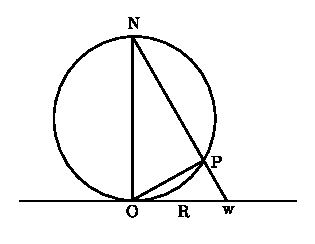
\includegraphics{hayman_fig2.eps}
\end{figure}

Consider the Riemann Sphere of diameter one lying over the $w$-plane
and touching it at $w=0$. To every point $w$ corresponds the point
$P(w)$ in which the line $Nw$ (fig) intersects the sphere. From the
figure $NP=\cos\theta=1/(1+R^{2})^{\frac{1}{2}}$, $R=|w|$. $NP$ is
called the chordal distance between $w$ and $\infty$ and is denoted by
$[w,\infty]$. 

Then\pageoriginale
$$
\frac{1}{2\pi}\int\limits^{2\pi}_{0}\log[1+|f(re^{i\theta})|^{2}]^{\frac{1}{2}}d\theta=\frac{1}{2\pi}\int\limits^{2\pi}_{0}\log\frac{1}{[f(z),\infty]}d\theta
$$
and so is the average of the chordal distances between $f(z)$ and
infinity, when $z$ runs over $|z|=r$. The left hand side of the above
equation is an alternative for $m(r,f)$ in the sense that it differs
from $m(r,f)$ by less than $\frac{1}{2}\log 2$.

It is easy to see that if $ds$ is an element of length in the plane
and $d\sigma$ the corresponding element on the Riemann-sphere then
$d\sigma=ds/(1+R^{2})$. Hence if $du$ $dv$ is an element of area in
the $w$-plane, then the corresponding element of area on the sphere is
$du\ dv/(1+R^{2})^{2}$. If $dx\ dy$ is an element of area in
$z$-circle, $|z|<r$, its image in the $w$-plane is
$|f'(z)|^{2}dx\ dy$, since the element of length is multiplied by
$|f'(z)|$. Thus the element of area corresponding to $dx\ dy$ on the
Riemann-$w$-sphere is precisely
$|f'(z)|^{2}dx\ dy/[1+|f(z)|^{2}]^{2}$. Therefore, we interpret $\pi
A(r)$ as the area on the Riemann-$w$-sphere of the image, with due
count of multiplicity (the map $w=f(z)$ may not be one-one, and more
than one lement of arc $x$ in the $z$-plane may go into the same
element of arc $x$ in the $w$-plane) of $|z|<r$ by $w=f(z)$. Since the
area of the sphere is $\pi$, $A(r)$ itself being the area of the image
divided by the area of the sphere may be interpreted as the average
number of roots in $|z|<r$ of the equation $f(z)=w$, as $w$ moves over
the Riemann sphere.

\subsubsection{}\label{part1-subsubsec1.6.2}\pageoriginale

We have seen above that $A(r)=\dfrac{1}{\pi}$ area of image of $|z|<r$
by $f(z)$ on the Riemann Sphere. So that $A(r)$ can be interpreted as
the average value of the number $n(r,a)$ of roots of $f(z)=a$, in
$|z|<r$ as $\ub{a}$ runs over the complex plane.

Let us now rotate the sphere. This corresponds to a one-one conformal
map of the closed plane onto itself and in fact to a bilinear map of
the type $w'=e^{i\lambda}(1+\ob{a}w)/(w-a)$ (for the proof refer
Carath\'eodery, \cite{1}). Further under this rotation $A(r)$ will
remain unaltered.

Set $\varphi(z)=e^{i\lambda}[1+\ob{a}f(z)]/[f(z)-a]$, and observe that
$[\varphi(z),\infty]=[f(z),a]$, where $w$, $a$ is the chordal distance
between the points corresponding to $w$ and $a$ on the Riemann
Sphere. In particular $[w,\infty]=\{1+|w|^{2}\}^{\frac{1}{2}}$. If we
apply our previous result to $\varphi(z)$, we get
\begin{align*}
\int\limits^{r}_{0}A(t) \frac{dt}{t} &=
N(r,\varphi)+\frac{1}{2\pi}\int\limits^{2\pi}_{0}\log\frac{1}{[\varphi(re^{i\theta}),\infty]}d\theta-\log\frac{1}{[\varphi(0),\infty]}\\
&=
N(r,a)+\frac{1}{2\pi}\int\limits^{2\pi}_{0}\log\frac{1}{[f(re^{i\theta}),a]}d\theta-\log
\frac{1}{[f(0),a]}.
\end{align*}
Thus we have proved the theorem.

\setcounter{dashthm}{1}
\begin{dashthm}\label{part1-thm2'}
For every complex $a$ and $a=\infty$
$$
\int\limits^{r}_{0}A(t)\frac{dt}{t}=N(r,a)+\frac{1}{2\pi}\int\limits^{2\pi}_{0}\log
\frac{1}{[f(re^{i\theta}),a]}d\theta-\log \frac{1}{[f(0),a]}.
$$
The\pageoriginale new chordal distance is
$$
[w,a]=\frac{1}{\left[1+\left|\dfrac{1+\ob{a}w}{w-a}\right|^{2}\right]^{\frac{1}{2}}}=\frac{|w-a|}{[(1+|a|^{2})(1+|w|^{2})]^{\frac{1}{2}}} 
$$
Thus in this above theorem, the expression $m_{0}(r,a)$ replaces
$m(r,a)$ of the Theorem \ref{part1-thm2'}, where,
$$
m_{0}(r,a)=\frac{1}{2\pi}\int\limits^{2\pi}_{0}\frac{\log[(1+|a|^{2})(1+|f(re^{i\theta})|^{2})]^{\frac{1}{2}}}{|f(re^{i\theta})-a|}d\theta
$$
Unlike theorem \ref{part1-thm2'} theorem \ref{part1-thm2'}' is
exact. Notice that $m_{0}(r,a)$ is always non-negative because the
chordal distance between any two points is always is less or equal to one.
\end{dashthm}

\begin{coro*}
If $f(z)$ is meromorphic in the plane then
$$
\int\limits^{r}_{1}n(t,a)\frac{dt}{t}\leq
\int\limits^{r}_{1}A(t)\frac{dt}{t}+C.
$$
for all $a$ where $C$ is independent of $a$ and $r(>1)$ but may depend
on $f$.
\end{coro*}

\begin{proof}
\begin{align*}
\int\limits^{r}_{0}A(t)\frac{dt}{t} &=N(r,a)+m_{0}(r,a)-m_{0}(0,a)\\
\int\limits^{1}_{0}A(t)\frac{dt}{t} &= N(1,a)+m_{0}(1,a)-m_{0}(0,a)
\end{align*}
subtracting, since $N(r,a)=\int\limits^{r}_{0}n(t,a)\dfrac{dt}{t}$, 
\begin{align*}
\int\limits^{r}_{1}n(t,a)\frac{dt}{t} &=\int\limits^{r}_{1}A(t)\frac{dt}{t}+m_{0}(1,a)-m_{0}(r,a)\\
&\leq \int\limits^{r}_{1}A(t)\frac{dt}{t}+\max\limits_{a}m_{0}(1,a)
\end{align*}\pageoriginale
since $m_{0}(r,a)$ is greater or equal to zero.

The maximum on the right is finite. In fact, for variable $\ub{a}$ and
fixed $r\,m_{0}(r,a)$ is continuous in $\ub{a}$ and is bounded as
$\ub{a}$ moves over the Riemann sphere. This is evident if the
function $f(z)\neq \ub{a}$ on $|z|=r$. If $f(z)=a$, at a finite number
of points the argument is similar to that in the Poisson-Jensen
formula. Putting $C=\Max\limits_{a}m_{0}(1,a)$ the result is obtained.
\end{proof}

\begin{remark*}
By an inequality for real positive functions due to W.K.\@ Hayman and
F.M.\@ Stewart \cite{1} and using corollary \ref{part1-coro1} we
deduce that if $f(z)$ is meromorphic and not constant in the plane and
$$
n(r)=\sup\limits_{a}\cdot n(r,a)\quad\text{and}\quad \epsilon>0,
$$
then
\begin{equation*}
n(r)<(e+\epsilon)A(r)\ldots\quad
\ldots\quad\ldots\tag{1.8}\label{part1-eq1.8} 
\end{equation*}
on a set $E$ of $r$ having the following property. If $E(r)$ is the
part of $E$ in $[1,r]$ then $\int\limits_{E(r)}\dfrac{dt}{t}\geq
c(\epsilon)\log r$ for all large $r$, where $c(\epsilon)$ depends only
on $\epsilon$.
\end{remark*}

The following are some open problems:
\begin{enumerate}
\renewcommand{\theenumi}{\alph{enumi}}
\renewcommand{\labelenumi}{(\theenumi)}
\item Can $e$ be replaced by a smaller constant and in particular by
  one in \eqref{part1-eq1.8}?

\item Does\pageoriginale \eqref{part1-eq1.8} hold for all large $r$;
  or for all large $r$ except a small set?

\item Can we assert
$$
\int\limits^{r}_{1}n(t)\frac{dt}{t}<\text{ (constant). } A(r)
$$
for some arbitrarily large $r$?
\end{enumerate}

\subsection{Functions in the plane}\label{part1-sec1.7}\pageoriginale

Let $S(r)$ be a real function $\geq 0$, and increasing for $0\leq
r\leq \infty$. The {\em order} $k$ and the {\em lower order} $\lambda$
of the function $S(r)$ are defined as
\begin{equation*}
\left.
\begin{matrix}
k\\
\lambda
\end{matrix}\right\}
=\mathop{\ob{\ub{\lim}}}_{r\to \infty}[\log S(r)]/\log r.
\end{equation*}
The order and the lower orders of the function always satisfy the
relation, $0\leq \lambda\leq k\leq \infty$.

If $0<k<\infty$, we distinguish the following possibilities,
\begin{itemize}
\item[(a)] $S(r)$ is maximal type if
$$
C=\ob{\lim}S(R)/R^{k}=\text{ infinity.}
$$

\item[(b)] $S(r)$ is of mean type of order $k$ if $0<C<\infty$.

\item[(c)] $S(r)$ is of minimal type if $C=0$.

\item[(d)] $S(r)$ is of convergence class if,
$$
\int\limits^{\infty}_{1}S(t)dt/t^{k+1}\quad \text{converges}.
$$
\end{itemize}
Note that if $S(r)$ is of order $k$ and $\epsilon>0$,
$$
S(r)<r^{k+\epsilon}\text{ \ for all large \ } r.
$$
and
$$
S(r)>r^{k-\epsilon} \text{ \ for some large \ } r.
$$
(This follows from the definition of order of $S(r)$.)

It can be seen that if $S(r)$ is of order $k$ and of convergence type
\iec (d) then it is of minimal type, (c). In fact in this case 
$$
\int\limits^{\infty}_{r_{0}}\frac{S(r)}{r^{k+1}}dr<\epsilon\quad\text{if}\quad
r_{0}>t(\epsilon)
$$\pageoriginale
Then 
$$
\int\limits^{2r_{0}}_{r_{0}}\frac{S(r)}{r^{k+1}}dr<\epsilon
$$
and since $S(r)$ increases with $r$,
$$
\int\limits^{2r_{0}}_{r_{0}}\frac{S(r)}{r^{k+1}}dr\geq
\frac{S(r_{0})}{(2r_{0})^{k+1}}r_{0}
$$
and
$$
S(r_{0})2^{-(k+1)}/r_{0}k<\epsilon\quad\text{for}\quad
r_{0}>t(\epsilon)
$$
that is,
$$
\mathop{\ob{\lim}}\limits_{r\to\infty} S(r)/r^{k}=0.
$$
So if (d) holds $S(r)$ is of minimal type. We also note that if $k'$
is greater than the order of $S(r)$ then,
$$
\int\limits^{\infty}_{1}S(r)dr/r^{k'+1}\quad\text{converges.}
$$
and if $k'$ is less than
$k\,\int\limits^{\infty}_{1}\dfrac{S(r)}{r^{k'+1}}dr$ diverges.

\subsubsection{We have next}\label{part1-subsubsec1.7.1}  

\begin{thm}\label{part1-thm4}
If $f(z)$ is a regular function for $|z|\leq R$ and 
\begin{gather*}
M(r,f)=\Max\limits_{|z|=r}f(z)\quad\text{then,}\\
T(r,f)\leq \log^{+}M(r,f)\leq
\frac{r+R}{R-r}T(R,f)\quad\text{for}\quad 0<r<R.
\end{gather*}
\end{thm}

\begin{proof}
Since $f(z)$ is regular in $|z|\leq R$ and $r<R$ we have, 
\begin{align*}
T(r,f)=T(r) &=
m(r,f)=\frac{1}{2\pi}\int\limits^{2\pi}_{0}\log^{+}|f(re^{i\theta})|d\theta\\
&\leq \frac{1}{2\pi}\Max\limits_{|z|=r}\log^{+}|f(re^{i\theta})|2\pi\\
&= \log^{+}M(r,f)
\end{align*}\pageoriginale
To prove the other side of the above inequality of the theorem we
distinguish between the two cases (i) $M(r)<1$ or (ii) $M(r)\geq
1$. In the case (i), $\log^{+}M(r)=0$ and $T(r,f)\times (R+r)/(R-r)$
being non-negative the inequality holds good. Hence we can now suppose
that $M(r)\geq 1$, and in which case $\log^{+}M(r)=\log M(r)$.

The Poisson-Jensen formula gives, for $z=re^{i\theta}$
\begin{gather*}
\log
|f(z)| = \frac{1}{2\pi}\int\limits^{2\pi}_{0}\log|f(Re^{i\phi})|\frac{(R^{2}-r^{2})}{R^{2}+2Rr\cos(\phi-\theta)+r^{2}}d\phi.\\
-\sum \log^{+}\left|\frac{(R^{2}-\ob{a}_{\mu} z)}{R(z-a_{\mu})}\right|
\end{gather*}
in the above equality $a_{\mu}$ runs through all the zeros of
$f(z)$. For, as regards the zeros with modulus less or equal to $R$
$$
\log^{+}\left|\frac{(R^{2}-\ob{a}_{\mu}z)}{R(z-a_{\mu})}\right|=\log
\left|\frac{(R^{2}-\ob{a}_{\mu}z)}{R(z-a_{\mu})}\right|\text{ \ since
  \ } \left|\frac{(R^{2}-\ob{a}_{\mu}z)}{(z-a_{\mu})R}\right|\geq
\ub{1}.
$$
and for the zeros $a \mu$ with modulus greater than $R$,
$$
\log^{+}\left|\frac{(R^{2}-\ob{a}_{\mu}z)}{R(z-a_{\mu})}\right|=0
$$
and Poisson's formula is unaffected.
\end{proof}

Clearly,
\begin{gather*}
\log|f|\frac{(R^{2}-r^{2})}{R^{2}-2Rr\cos(\phi-\theta)+r^{2}} \leq
\log^{+}|f|\frac{(R^{2}-r^{2})}{R^{2}-2Rr\cos (\phi-\theta)+r^{2}}\\
\leq \frac{R+r}{R-r}\log^{+}f \;
-\;\frac{R+r}{R-r}\log^{+}f
\end{gather*}\pageoriginale
\begin{align*}
\log|f(z)| &\leq
\frac{1}{2\pi}\int\limits^{2\pi}_{0}\frac{(R^{2}-r^{2})}{(r^{2}+R^{2}-2Rr)}\log^{+}|f(Re^{i\phi})|d\phi\\
&
=(1/2\pi)\int\limits^{2\pi}_{0}(R+r/(R-r))\log^{+}|f(Re^{i\phi})|d\phi\\
\log|f(z)| &\leq (R+r/(R-r)) T(R,f).
\end{align*}
This being true for all $z$, $|z|=r$, holds good for the $z$ at which
$f(z)$ takes the maximum $M(r,f)$.

Hence,
$$
\log M(r,f)\leq (\ob{R+r}/\ob{R-r})T(R,f).
$$

\begin{coro*}
If $f(z)$ is an integral function, the order and type ($a$, $b$, $c$
or $d$ defined in the last article) of $T(r)$ and $\log^{+}M(r)$ are
the same.
\end{coro*}

From the left hand side of the inequality of Theorem \ref{part1-thm4},
it follows that the order and type of $T(r,f)$ are not bigger than
those of $\log^{+}M(r)$. In order to prove the reverse, let us
substitute $R=2r$ in the right side of the theorem. We get,
$$
\log^{+}M(r,f)\leq 3T(2r,f)
$$
Suppose $k$ is the order of $T(r,f)$, then given $\epsilon>0$,
$T(r,f)<\epsilon r^{k+\epsilon}$ for all $r>r_{0}$ by the definition
of order. Hence combining the two inequalities,
$$
\log^{+}M(r,f)\leq 3T(2r,f)<3 \epsilon
(2r)^{k+\epsilon}\quad\text{for}\quad r>r_{0}.
$$
This implies that the order of $\log^{+}M(r,f)$ is less or equal to
$k$. If $T(r)$ has mean type, we may take $\epsilon=0$. If $T(r)$ has
minimal type, we\pageoriginale may in addition take $c$ arbitrarily
small. Hence $T(r,f)$ and $\log^{+}M(r,f)$ both have same order and
belong to the same order type $a$, $b$ or $c$. In order to complete
the corollary, we have to consider the case when $T(r,f)$ is of (d)
\iec convergence type. Consider,
\begin{gather*}
\int\limits^{\infty}_{r_{0}}\frac{\log^{+}M(r)}{r^{k+1}}dr\\
\int\limits^{\infty}_{r_{0}}\frac{\log^{+}M(r)}{r^{k+1}}dr\leq 
\int\limits^{\infty}_{r_{0}}\frac{3T(2r)}{r^{k+1}}dr
\end{gather*}
$k$ being the order of $T(r,f)$.
$$
=\int\limits^{\infty}_{2r_{0}}3.2^{k}\frac{T(r)dr}{r^{k+1}}
$$
by change of variable.

Since $T(r)$ is of convergence type, it follows from the above
inequality that $\log^{+}M(r)$ also belongs to the same class. It is
clear that this relation holds good in the reverse direction.

We now proceed to define the order and the order type of a function
$f(z)$ meromorphic in the plane on the above analogy.

\begin{defi*}
The {\em order} and {\em type} of a function $\ub{f(z)}$ {\em
  meromorphic} in the plane are {\em defined} as the {\em order} and
{\em type of $\ub{T(r,f)}$.} 
\end{defi*}

We note that this coincides with that of order and type of\break
$\log^{+}M(r,f)$ if $f(z)$ is an entire function.

\subsubsection{}\label{part1-subsubsec1.7.2}

\begin{example*}
\begin{enumerate}
\renewcommand{\labelenumi}{(\theenumi)}
\item If the function $f(z)=e^{z}$, $\log M(r)=r$ and
  $T(r)=r/\pi$.\pageoriginale The function has order one, mean
  type. In this case $\log^{+}M(r)$ and $T(r)$ are of the same type,
  viz., mean type, though the values of the type are different. More
  precisely, for $T(r)$,
  $\mathop{\ob{\lim}}\limits_{r\to\infty}T(r)/r=1/\pi$ (the order
  being $1$) and for $\log^{+}M(r)$, $\mathop{\ob{\lim}}\limits_{r\to
    \infty}(1/r)\log^{+}M(r)=1$. 
\end{enumerate}
\end{example*}

In the above example the ratio of the two super.\@ limites that is,
$$
\frac{\lim\limits_{r\to\infty}\dfrac{T(r)}{r^{k}}}{\lim\limits_{r\to
    \infty}\dfrac{\log^{+}M(r)}{r^{k}}}=1 
$$
In general case for a function of order $k$ and mean type this ratio
is bounded by $1$. But it is still an open problem to find the best
possible lower bound. It can be shown easily from theorem
\ref{part1-thm4}, taking \break $R=r[1+(1/k)]$, that a lower bound is
$1/e(2k+1)$. In this connection P.B.\@ Kennedy \cite{1} has given a
counter example of a function of order $k$ mean type in $|\arg
z|<\pi/2k$, and bounded for $\pi/2k\leq \arg z\leq \pi$, provided
$k>\frac{1}{2}$, such that
\begin{align*}
& \log^{+}|f(re^{i\theta})|\sim r^{k}\cos k\theta \quad\text{for}\quad
  |\theta|<\pi/2k\\
& \log^{+}|f(re^{i\theta})|=0(1)\quad \frac{\pi}{2k}\leq |\theta|<\pi
\end{align*}
Hence $T(r,f)\sim r^{k}/k$, $\log M(r)\sim r^{k}$. Thus $e(2k+1)$
cannot be replaced by any constant less than $k\pi$ if $k>\frac{1}{2}$.

\begin{remark*}
For functions of infinite order $T(r)$ and $\log^{+}M(r)$ no longer
have necessarily the same order of magnitude. Actually it has been
shown by W.K.\@ Hayman and F.M.\@ Stewart \cite{1} that if $\epsilon
>0$, $\log M(r)<(2e+\epsilon)[T(r)+A(r)]$\pageoriginale for some large
$r$. As an example consider $f(z)=e^{e^{z}}$
$$
\log M(r)=e^{r}
$$
and
$$
T(r)\sim e^{r}(2\pi^{3})^{\frac{1}{2}}/r^{\frac{1}{2}}.
$$
\end{remark*}

\subsection[Representation of a function....]{Representation of a function in terms of its zeros and
  poles}\label{part1-sec1.8}

\pageoriginale
\begin{defi*}
For any complex number $z$, and any integer $q>0$,
$$
E(z,q)=(1-z)e^{z+\frac{1}{2}z^{2}+\cdots+\frac{1}{q}z^{q}}.
$$
\end{defi*}

\begin{thm}[Nevanlinna]\label{part1-thm5}
If $f(z)$ is meromorphic in the plane with zeros $a_{\mu}$ and poles
$b_{\nu}$ and $f(z)$ being of order at most $q$ of the minimal type
then,
$$
f(z)=z^{p}e^{P_{q-1}(z)}\lim\limits_{R\to
  \infty}\frac{\prod\limits_{1a_{\mu}|<R} E\left(\dfrac{z}{a_{\mu}},
  q-1\right)}{\prod\limits_{1b_{\mu}|<R} 
  E\left(\dfrac{z}{b_{\nu}},q-1\right)} 
$$
where $p$ is a suitable integer and $P_{q-1}(z)$ is a polynomial of
degree at most $q-1$.
\end{thm}

Note that the theorem only asserts that the limit on the right exists,
but it does not indicate whether the products are convergent or
divergent.

In fact if $f(z)$ only satisfies the weaker condition that lower limit
as $r$ tends to infinity of $T(r)/r^{q}$ is equal to zero (instead of
the condition assumed in the theorem viz., upper limit of the same is
zero.), the result still holds provided that $R$ is allowed to tend to
infinity through a suitable sequence of values, instead of all values.

To start with let us assume that the function $f(z)$ has no
zero\pageoriginale or pole at zero. The Poisson-Jensen formula gives,
\begin{align*}
& \log |f(z)|=\frac{1}{2}\pi
\int\limits^{2\pi}_{0}\frac{(R^{2}-r^{2})\log
  |f(Re^{i\phi})|}{R^{2}-2Rr\cos(\phi-\theta)+r^{2}}d\phi +
\sum\limits_{|a_{\mu}|<R}\log \left|
\frac{R(z-a_{\mu})}{(R^{2}-\ob{a}_{\mu}z)}\right|\\ 
&\hspace{2cm} z=re^{i\theta}\hspace{3.47cm} +\sum_{|b_{\nu}|<R}\log
\left|\frac{R^{2}-\ob{b}_{\nu}z}{R(z-b_{\nu})}\right| 
\end{align*}
Both the sides are equal harmonic functions $v(z)$ (say) of $z$ near
the point $z=re^{i\theta}$ where $f(re^{i\theta})\neq 0$,
$\infty$. Let us operate $\dfrac{\partial v}{\partial
  x}-i\dfrac{\partial v}{\partial y}$ on both the sides. We assume
that $R$ is such that $f(z)\neq 0$, $\infty$ on
$|z|=R$. Differentiating under the integral sign and observing that
$$
\Real 
\left(\frac{Re^{i\phi}+z}{Re^{i\phi}-z}\right) =
\frac{(R^{2}-r^{2})}{R^{2}-2Rr\cos(\phi-\theta)+r^{2}}  
$$
We deduce,
\begin{align*}
& \frac{f'(z)}{f(z)}=\frac{1}{2\pi}\int\limits^{2\pi}_{0}\log|f(Re^{i\phi})|\frac{2Re^{i\phi}}{(Re^{i\phi}-z)}d\phi\\
&\qquad\qquad
-\sum_{|a_{\mu}|<R}\left[\frac{1}{(a_{\mu}-z)}-\frac{\ob{a}_{\mu}}{(R^{2}-\ob{a}_{\mu}z)}\right]\\
&\qquad\qquad
+\sum_{|b_{\nu}|<R}\left[\frac{1}{(b_{\nu}-z)}-\frac{\ob{b}_{\nu}}{(R^{2}-\ob{b}_{\nu}z)}\right] 
\end{align*} 
provided\pageoriginale that there are no zeros or poles on
$|z|=R$. Differentiating this $q-1$ times,
\begin{align*}
\left(\frac{d}{dz}\right)^{q-1} \left(\frac{f'(z)}{f(z)}\right) &
=\frac{1}{\pi}\int\limits^{2\pi}_{0}\frac{\log
  |f(Re^{i\phi})|Re^{i\phi}}{(Re^{i\phi}-z)^{q+1}}\\ 
&\quad +(q-1)\sum_{|b_{\nu}|<R}\left(\frac{1}{(b_{\nu}-z)^{q}}-\frac{\ob{b}_{\nu}^{q}}{(R^{2}-\ob{b}_{\nu}z)^{q}}\right)\\
&\quad +(q-1)\sum_{|a_{\mu}|<R}\left(\frac{1}{(a_{\mu}-z)^{q}}-\frac{\ob{a}^{q}_{\mu}}{(R^{2}-z\ob{a}_{\mu})^{q}}\right)
\end{align*}
Suppose now that $T(2r)/(r)^{q}$ tends to zero as $r$ tends to
$\infty$ either through all values or through a suitable sequence of
values, say $R_{k}$ (which tends to $\infty$ with $k$). Such a
sequence of values exists by our assumptions. Also by decreasing
$R_{k}$ slightly if necessary we may assume that $f(z)\neq 0$,
$\infty$ on $z=R_{k}$, we take $R=R_{k}$ in (1).  

Then since $m(r,f)\geq 0$,
$$
T(2R_{k},f)\geq N(2R_{k},f)\geq
\int\limits^{2R_{k}}_{R_{k}}n(t,f)\frac{dt}{t}\geq n(R_{k},f)\log 2.
$$
Thus $n(R_{k},f)R^{q}_{k}$ tends to zero as $k$ tends to
$\infty$. Similarly, $n(R_{k},1/f)/R_{k}^{q}\unskip\break\to 0$, as $k\to \infty$)
since, $T(R_{k},1/f)=T(R_{k},f)+0(1)$ and $T(R_{k},f)/R_{k}^{q}\to
0$. Our aim now is to show that some of the terms on the right of the
equation 11.9 including the integral tend to zero uniformly for $z$ on
any bounded set as $k$ tends to infinity. Then letting $k$ tend to
infinity, we get a modified equation integrating which $q$ times we
will get the result.

Now\pageoriginale suppose that $|z|<\dfrac{1}{2}R_{k}$. Then,
$|\ob{b}_{\nu}z|<\dfrac{1}{2}R_{k}\cdot R_{k}$ for
$|b_{\nu}|<R_{k}$. and
$$
|R^{2}_{k}-\ob{b}_{\nu}z|\geq R^{2}_{k}-|b_{\nu}z|\geq
\dfrac{1}{2}R^{2}_{k}
$$
Hence,
$$
\left|\frac{\ob{b}^{q}_{\nu}}{(R^{2}_{k}-\ob{b}_{\nu}z)}\right|<\frac{R^{q}_{k}}{(\dfrac{1}{2}R^{2}_{k})^{q}}=\frac{2^{q}}{R^{q}_{k}}
$$
this inequality being true for all poles $b_{\nu}$ with
$|b_{\nu}|<R_{k}$. Therefore, summing up for all poles $b_{\nu}$,
$|b_{\nu}|<R_{k}$ 
$$
\left|\sum
\frac{\ob{b}^{q}_{\nu}}{(R^{2}_{k}-\ob{b}_{\nu}z)}\right|\leq
\sum\left|\frac{\ob{b}^{q}_{\nu}}{(R^{2}_{k}-\ob{b}_{\nu}z)^{q}}\right|<\frac{n(R_{k},f)2^{q}}{R^{q}_{k}} 
$$
and hence the right hand side tends to zero uniformly as $k$ tends to
infinity for $z$ in any bounded set. A similar result holds good in
the case of the zeros of the function.

Now coming to the integral,
$$
|R_{k}e^{i\phi}-z)|\geq \frac{1}{2}R_{k}\quad\text{for}\quad
|z|<\frac{1}{2}R_{k}.
$$
Hence the modulus of the integral on the right of \eqref{part1-sec1.9} is
at most,
\begin{align*}
& (q!)\frac{R_{k}}{\pi}\frac{2^{q+1}}{R^{q+1}_{k}}\int\limits^{2\pi}_{0}\left|\log
  |f(R_{k}e^{i\phi})|\right|d\phi\\
&\frac{(q!)}{\pi}\frac{2^{q+1}}{R^{q}_{k}}\left[\int\limits^{2\pi}_{0}\log^{+}|f(Re^{i\phi})|d\phi+\int\limits^{2\pi}_{0}\log^{+}\frac{1}{|f(Re^{i\phi})|}d\phi\right]\\
&< (q!)\frac{2^{q+2}}{R^{q}_{k}}[m(R_{k},f)+m(R_{k},1/f)]\\
&< (\text{Const.)}
  \frac{T(R_{k},f)}{R^{q}_{k}}<(\text{Const.})\frac{T(2R_{k},f)}{R^{q}_{k}}\to
  0\\
&\hspace{5.15cm} \text{as \ } k\to \infty.
\end{align*}\pageoriginale
Now the equation \eqref{part1-sec1.9} takes the form,
$$
\left(\frac{d}{dz}\right)^{q-1}\frac{f'(z)}{f(z)}=\lim\limits_{k\to\infty}S_{k}(z)
$$
Where
$$
S_{k}(z)=(q-1)!\left\{\sum_{|b_{\nu}|<R_{k}}\frac{1}{(b_{\nu}-z)}q-\sum_{|a_{\mu}|<R_{k}}\frac{1}{(a_{\mu}-z)}q\right\} 
$$
the convergence being uniform for any bounded set of values of $z$ not
containing any of the zeros or poles of $f(z)$.

By the uniform convergence we may therefore, integrate both sides
$(q-1)$ times along a suitable path from $0$ to $z$ to get,
\begin{multline*}
\frac{f'(z)}{f(z)}=\lim\limits_{k\to\infty}\left[\sum_{|b_{\nu}|<R_{k}}\left\{\frac{1}{(b_{\nu}-z)}-\frac{1}{b_{\nu}}-\frac{z}{b_{\nu}^{2}}-\cdots-\frac{z^{q-2}}{b^{q-1}_{\nu}}\right\}\right.\\
\left. -\sum_{|a_{\mu}|<R_{k}}\left\{\frac{1}{(a_{\mu}-z)}-\frac{1}{a_{\mu}}-\cdots-\frac{z^{q-2}}{a_{\mu}^{q-1}}\right\}\right]+p_{q-2}(z)
\end{multline*}
where $P_{q-2}(z)$ is a polynomial of degree at most $q-2$. Now
integrate both the sides once more from $0$ to $z$, and take
exponentials,
$$
f(z)=P_{q-1}(z)\lim\limits_{k\to
  \infty}\frac{\prod\limits_{|a_{\mu}|<R_{k}}
  \left(1-\dfrac{z}{a_{\mu}}\right) e^{\frac{z}{a_{\mu}} +
    \frac{z^{2}}{2a^{2}_{\mu}}+\cdots+\frac{z^{q-1}}{(q-1)a^{q-1}_{\mu}}}}
{\prod\limits_{|b_{\nu}| <R_{k}} \left(1-\dfrac{z}{b_{\nu}}\right)
  e^{\frac{z}{b_{\nu}} + \cdots\frac{1}{q-1}\left(\frac{z}{b_{\nu}}\right)^{q-1}}} 
$$
Hence\pageoriginale the result in the case when $f(0)\neq 0$,
$\infty$. In case zero is a pole or zero of the function of order $p$,
consider the function $f(z)/z^{p}$ and apply the result just obtained
to get the theorem in its final form.

\subsection{Convergence of Weierstrass
  products}\label{part1-sec1.9}\pageoriginale 

Let $a_{1}$, $a_{2},\ldots a_{n}\ldots$ be a sequence of complex
numbers (none $0$) with moduli $r_{1}$, $r_{2},\ldots,r_{n},\ldots$ in
the increasing order of magnitude. Let $n(r)$ be defined as
$$
n(r)=\mathop{\text{Sup.}}\limits_{r_{k}<r}k.
$$
Then follows the result:

\begin{lemma*}
If $N(r)=\int\limits^{r}_{0}\dfrac{n(t)}{t}dt$ then $N(r)$ and $n(r)$
have the same order and type; and for any $k$, such that $0<k<\infty$,
the series $\sum 1/r^{k}_{n}$ and the integrals
$\int\limits^{\infty}_{0}\dfrac{n(r)}{r^{k+1}}dr$, and
$\int\limits^{\infty}_{0}N(r)\dfrac{dr}{r^{k+1}}$ converge or diverge
together.
\end{lemma*}

\begin{proof}
By Riemann-Stieltjes' integrals,
\begin{align*}
\sum_{r_{n}<R}1/r_{n}^{k} &= \int\limits^{R}_{0}\frac{1}{t^{k}} \,dn (t)\\
&= k\int\limits^{R}_{0}n(t)\dfrac{dt}{t^{k+1}}+n(R)/R^{k} \text{
  \ because \ } n(t)=0
\end{align*}
near $0$. Suppose now
$I_{1}=\int\limits^{\infty}_{0}n(R)\dfrac{dR}{R^{k+1}}$ is less than
infinity. $n(R)$ has at most convergence type of order $k$. (Hence it
is also of minimal type). Therefore upper limit of $n(r)/r^{k}$ as $r$
tends to infinity =  zero, and $\sum 1/r^{k}_{n}$ converges to
$k(I_{1})$. The convergence of the series implies the convergence of
the integral, because $n(R)/R^{k}\geq 0$.
\end{proof}

Now\pageoriginale consider the integral,
\begin{align*}
\int\limits^{R}_{0}N(r) \frac{dr}{r^{k+1}} &=
N(R)/(-k)R^{k}+\int\limits^{R}_{0}dN(r)/kr^{k}\\
&= -N(R)/kR^{k}+\int\limits^{R}_{0}\frac{n(r)}{k}dr/r^{k+1} 
\end{align*}
From this inequality we get that the integrals
$\int\limits^{\infty}_{0}N(r)dr/r^{k+1}$ and\break
$\int\limits^{\infty}_{0}n(r)dr/r^{k+1}$ will converge or diverge
together, due to the following reason. The convergence of
$\int\limits^{\infty}_{0}N(r)\dfrac{dr}{r^{k+1}}$ implies that
$\mathop{\ob{\lim}}\limits_{R\to \infty}N(R)/R^{k}=0$, hence the convergence of
$\int\limits^{\infty}_{0}n(r)\dfrac{dr}{r^{k+1}}$ follows. On the
other hand if $\int\limits^{\infty}_{0}n(r)dr/r^{k+1}$ converges
$\int\limits^{R}_{0}N(r)\dfrac{dr}{r^{k+1}}$ at once by comparison.

Therefore it remains to be proved that $n(r)$ and $N(r)$ have the same
order and type. Suppose $n(r)$ has order $k$, then given $\delta>0$, 
$n(r)<c r^{k+\delta}$ for $r$ greater than $r_{0}$
\begin{align*}
N(r) &= \int\limits^{r}_{0}n(t)\dfrac{dt}{t}\\
&=
\int\limits^{r_{0}}_{0}n(t)\dfrac{dt}{t}+\int\limits^{r}_{r_{0}}n(t)\dfrac{dt}{t}\quad\text{for}\quad
r>r_{0}\\
N(r) &\leq
\int\limits^{r_{0}}_{0}n(t)\dfrac{dt}{t}+\int\limits^{r}_{r_{0}}cr^{k-1^{+}}\,
dr\text{ \  for \ } r>r_{0}\\
&\leq \text{ \ constant \ } +cr^{k+\delta}/(k+\delta)\text{ \  for \ } r>r_{0}.
\end{align*}

This implies that order of $N(r)$ is not greater than that of $n(r)$,
and if $n(r)$ has got mean or minimal type so has $N(R)$. The result
for convergence\pageoriginale or divergence class follows from earlier
inequalities. The estimate for $n(r)$ in terms of $N(r)$ follows from
$$
n(r)\leq (1/\log 2)\int\limits^{2r}_{r}n(t)\dfrac{dt}{t}\leq
N(2r)/\log 2.
$$
From this inequality it can be derived in the same way as before, that
the order of $n(r)$ is not greater than that of $N(r)$ etc.

\begin{defi*}
The order and type of $n(r)$ or $N(r)$ (being the same) are called the
order and type of the sequence $(a_{n})$. The order of $n(r)$ is also
sometimes called {\em exponent of convergence} of the sequence.
\end{defi*}

We note that $\sum 1/r_{n}^{k}$ converges if and only if $n(r)$ has
order less than $k$, or order $k$ of convergence type. (This is a
consequence of lemma~3)

\subsubsection{}\label{part1-subsubsec1.9.1}
Next let us state the theorem,

\begin{thm}\label{part1-thm6}
Suppose that $a_{n}$ is a sequence having at most order $q+1$ 
(a~positive integer) convergence class. Then the product
$\pi(z)=\prod\limits^{\infty}_{n=1}\unskip\break E(z/a_{n},q)$ converges absolutely
and uniformly in any bounded region, and for $|z|=r$,
$$
\log|\pi(z)|<A(q)\left\{r^{q}\int\limits^{r}_{0}n(t)\dfrac{dt}{t^{q+1}}+r^{q+1}\int\limits^{\infty}_{0}n(t)\dfrac{dt}{t^{q+2}}\right\}
$$
\end{thm}

\begin{proof}
\begin{align*}
E(u,q) &= (1-u)e^{u+\frac{1}{2}u^{2}+\cdots+\frac{u^{q}}{q}}\\
\log \ E(u,q) &= \log(1-u)+u+\frac{1}{2}u^{2}+\cdots+\frac{u^{q}}{q}\\
&= -\sum_{q+1}u^{k}/k
\end{align*}
so\pageoriginale that $|\log
E(u,q)|-\sum\limits_{q+1}\dfrac{|u|^{k}}{k}\leq 2|u|^{q+1}$ if
$|u|\leq \dfrac{1}{2}$ since $\log|E(u,q)|$ is the real part of $\log
E(u,q)$ we get $\log|E(u,q)|\leq q+1$ if $|u|\leq
\dfrac{1}{2}$. Suppose $\dfrac{1}{2}\leq |u|\leq 1$. Then 
\begin{align*}
\log |E(u,q)| &\leq
\log|(1-u)|+|u|+\frac{1}{2}|u|^{2}+\cdots+\dfrac{|u|^{q}}{q}\\
&\leq |u|+|u|+\frac{1}{2}|u|^{2}+\cdots+\frac{|u|^{q}}{q}.
\end{align*}
Also $|u|\geq \dfrac{1}{2}$, $|u|^{q-1}\geq 1/2^{q-1}$,
$2^{q-1}|u|^{q-1}\geq |u|$. So that since $|u|\leq 1$, $|u|^{q}\leq
|u|\leq 2^{q-1}|u|^{q}$ and 
$$
\log|E(u,q)|\leq 2^{q-1}|u|^{q}+q2^{q-1}|u|^{q}=A(q)|u|^{q}<2A(q).
$$
$A(q)$ being a constant depending only on $q$. 

Thus for $|u|\leq 1$,
$\log|E(u,q)|\leq A(q)|u|^{q+1}$.
\end{proof}

Let
\begin{align*}
|u|\geq 1, \text{ \ then \ } \log |E(u,q)| &\leq
|u|+|u|+\frac{1}{2}|u|^{2}+\cdots+\frac{u^{q}}{q}\\
&\leq (q+1)|u|^{q} 
\end{align*}
Now $u=z/z_{n}$. Let $|z|=r$, $|z_{n}|=r_{n}$ and $N$ the least
integer for which $r_{n}\geq r$. Then $|u|\geq 1$. Thus
$$
\sum^{N-1}_{n=1}\log |E(z/z_{n},q)|\leq
A(q)r^{q}\sum^{N-1}_{1}r^{-q}_{n}
$$
and
$$
\sum^{\infty}_{n+1}\log E(z/z_{n},q)\leq
B(q)r^{q+1}\sum^{\infty}_{n+1}r^{-q-1}_{n} 
$$
Thus 
\begin{align*}
\sum^{\infty}_{1}\log |E(z/z_{n},q)| &\leq
C\left[r^{q}\sum^{N-1}_{1}r^{-q}_{n}+r^{q+1}\sum^{\infty}_{N}r^{-q-1}_{n}\right]\\
&=
C\left[r^{q}\int\limits^{r}_{0}\frac{1}{t^{q}}dn(t)+r^{q+1}\int\limits^{\infty}_{r}\frac{1}{t^{q+1}}dn(t)\right]
\\
&= K\left[r^{q}\int\limits^{r}_{0}\frac{1}{t^{q+1}}n(t)dt+r^{q+1}\int\limits^{\infty}_{r}\frac{1}{t^{q+2}}n(t)dt\right]
\end{align*}\pageoriginale
$K$ depending only on $q$. This proves the theorem.

We also see that for large $n$,
$$
\left|\log
E\left(\frac{z}{z_{n}},q\right)\right|<A(q)\left(\frac{r}{r_{n}}\right)^{q+1},
$$
and, the product converges since $\sum r^{-(q+1)}_{n}$ converges. Our
Theorem \ref{part1-thm6} shows that if in Theorem \ref{part1-thm5}
$f(z)$ has at most order $q$ convergence class, then the two products
converge separately, uniformly and absolutely on every bounded set.

\subsubsection{As a consequence of the theorem we
  have}\label{part1-subsubsec1.9.2} 

\begin{thm}\label{part1-thm7}
If a sequence $a_{n}$ defined as in the last theorem, has order
$\rho$, $q-1\leq \rho<q$, $q$ an integer, then
$\pi_{a}(z)=\prod\limits^{n=\infty}_{n=1}E(z/a_{n},q-1)$ has order
$\rho$ and further if $\rho$ is not an integer, $\prod\limits_{a}(z)$
has the same type class as $(a_{n})$.
\end{thm}

Hence if $f(z)$ is meromorphic of finite non-integral order, then the
roots of $f(z)=a$, have the same order and type class as $f(z)$ except
for at most one value of $\ub{a}$ on the Riemann sphere.

\begin{proof}
If $n(t)<ct^{\rho+\epsilon}$ for $t> t_0$ where $\epsilon>0$
\begin{align*}
& r^{q-1}\int\limits^{r}_{0}n(t)\frac{dt}{t^{q}}\leq
  r^{q-1}\int\limits^{t_{0}}_{0}n(t)dt/t^{q}+r^{q-1}\int\limits^{r}_{t_{0}}ct^{\rho+\epsilon}dt/t^{q}\\
&\quad
  -0(r^{q-1})+C\frac{r^{\rho+1-q+\epsilon}}{\rho+1+-q+\epsilon}r^{q-1}=0\left(r^{q-1}+\frac{Cr^{\rho+\epsilon}}{\rho+\epsilon+1-q}\right)
\end{align*}\pageoriginale
and the result regarding the order of the first integral follows. The
second integral is treated similarly and then the first part follows
from Theorem \ref{part1-thm6}.

If $\rho>q-1$ and $f(z)$ is of mean type or minimal type of order
$\rho$ we can take $\epsilon=0$, and in the case of minimal type $c$
small and the results for the type at once follow. Suppose for
instance that $n(t)$ has order less than $q$ so that
$n(t)<cr^{\rho+\epsilon}$ for $t>t_{0}$. Then for large $r$,
$$
r\int\limits^{\infty}_{r}\frac{n(t)dt}{t^{q+1}} <
cr^{q}\int\limits^{\infty}_{r}\frac{t^{\rho+\epsilon}}{t^{q+1}}dt=\frac{cr^{\rho+\epsilon}}{(q-\rho-\epsilon)}\quad\text{if}\quad
\epsilon<q-\rho. 
$$
and the integral is $0(r^{\rho+\epsilon})$ and is $0(r^{\rho})$ if
$n(r)=0(r^{\rho})$ as required.
\end{proof}

Suppose now that $f(z)$ is a meromorphic function of finite
non-integral order $\rho$ and $q$ such that $q-1<\rho<q$. Then,
$$
f(z)=e^{P_{q-1}(z)}\Pi_{1}(z)/\Pi_{2}(z)
$$
where $\Pi_{1}(z)$ and $\Pi_{2}(z)$ are the products over the zeros
and poles respectively. Now if both have a smaller order and type than
$f(z)$, so does their ratio. since\pageoriginale
\begin{align*}
T(r,\Pi_{1}/\Pi_{2}) &\leq T(r,\Pi_{1})+T(r,1/\Pi_{2})\\
&= T(r,\Pi_{1})+T(r,\Pi_{2})+0(1).
\end{align*}
and $e^{P_{q-1}(z)}$ has order $q-1<\rho$, so we should get a
contradiction. Hence at least one of the $\Pi_{1}(z)$ or $\Pi_{2}(z)$
and so either zeros or the poles have the same order and type as the
function $f(z)$.
 
If for instance the poles do not have the order and type of $f(z)$
then since $f(z)-a$ has the same poles as $f(z)$ (for every finite
$a$), the roots of $f(z)=a$ that is the zeros of $f(z)-a$ have the
order and type of $f(z)$.

This kind of argument was used to show that Riemann-Zeta function has
an infinity of zeros.

We now illustrate the above by means of an example.

If $f(z)$ is meromorphic in the plane and
$\mathop{\ub{\lim}}\limits_{\mu\to\infty}T(r,f)/\log r^{<+\infty}$
then $f(z)$ is rational.

In this case $f(z)$ has lower order zero, and lower limit of
$N(r,f)/\unskip\break\log r$ as $r$ tends to $\infty$ is less than
$\infty$. $[T(r,f)\geq N(r,f)]$.

Similarly,
$$
\mathop{\ub{\lim}}\limits_{\nu\to\infty}\frac{N(r,1/f)}{\log r}<\infty
$$
further,
$$
N(R,f)\geq \int\limits^{R}_{r}n(t,f)\frac{dt}{t}\geq
n(r,f)\log\frac{R}{r}
$$
so that $n(r,f)\leq \dfrac{N(r^{2},f)}{\frac{1}{2}\log r}=0(1)$ for a
sequence of $n\to \infty$. So $f(z)$ has only a finite number of zeros
and poles. Hence from theorem \ref{part1-thm5}\pageoriginale 
$f(z)=z^{p}(\Pi(1-z/a_{\mu})/(1-z/b_{\nu})$ where both the products are
finite. Thus for all transcendental meromorphic functions
$T(r,f)/\log r$ tends to infinity as $r$ tends to infinity.




